\documentclass[a4paper,14pt]{article}

\usepackage{cmap}
\usepackage[T2A]{fontenc}
\usepackage[utf8]{inputenc}
\usepackage[english,russian]{babel}

\title{Отчет по заданию в Kaggle}
\author{Гончарова Наталия, группа БПМ-17-2}
\date{Декабрь 2020 г.}

\usepackage{natbib}
\usepackage{graphicx}
\graphicspath{./pics/}

\begin{document}

\maketitle

\section{Постановка задачи}
Решение задачи с Kaggle с исползованием нейронной сети.
Ссылка на задачу - \textbf{https://www.kaggle.com/nasa/kepler-exoplanet-search-results}

\section{Входные переменные}
Ознакомимся со структурой файла \textbf{kepler-exoplanet-search-results.csv}

\begin{figure}[h!]
\centering
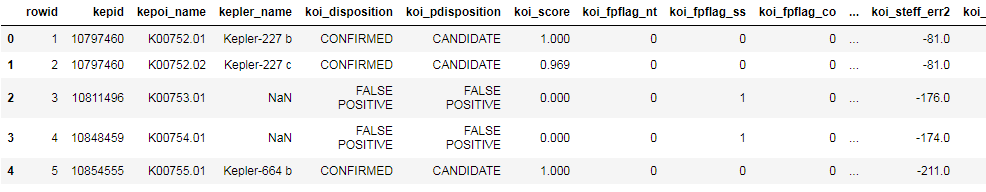
\includegraphics[scale=0.6]{pics/1.png}
\caption{Cтруктура файла}
\end{figure}

\section{Решение}
Посмотрим на распределение параметров \textbf{koi-pdisposition} и \textbf{koi-disposi}.

\begin{figure}[h]
\begin{minipage}[h]{0.5\linewidth}
\center{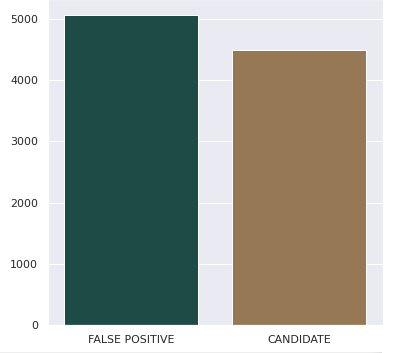
\includegraphics[width=0.5\linewidth]{pics/2.png} \\ а)}
\end{minipage}
\hfill
\begin{minipage}[h]{0.5\linewidth}
\center{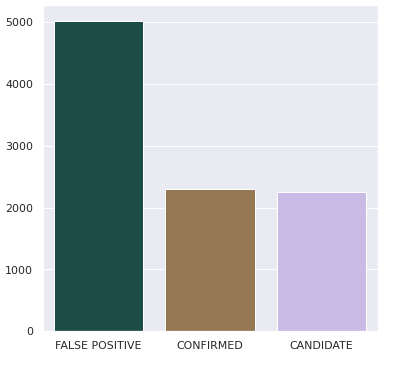
\includegraphics[width=0.5\linewidth]{pics/3.png} \\ б)}
\end{minipage}
\caption{Распределение параметров}
\end{figure}

Перекодируем категориальные признаки для дальнейшего анализа. Реализуем функцию, которая принимает на вход DataFrame, кодирует числовыми значениями категориальные признаки и возвращает обновленный DataFrame и сами кодировщики.

\begin{figure}[h!]
\centering
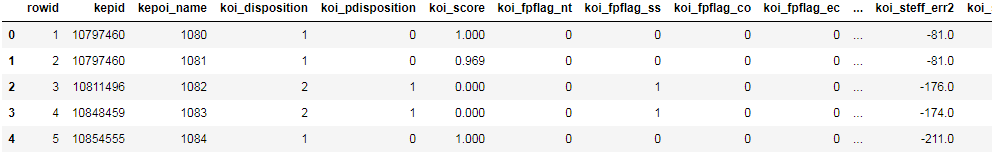
\includegraphics[scale=0.6]{pics/4.png}
\caption{Категориальные признаки}
\end{figure}

Построим матрицу корреляций:

\begin{figure}[h!]
\centering
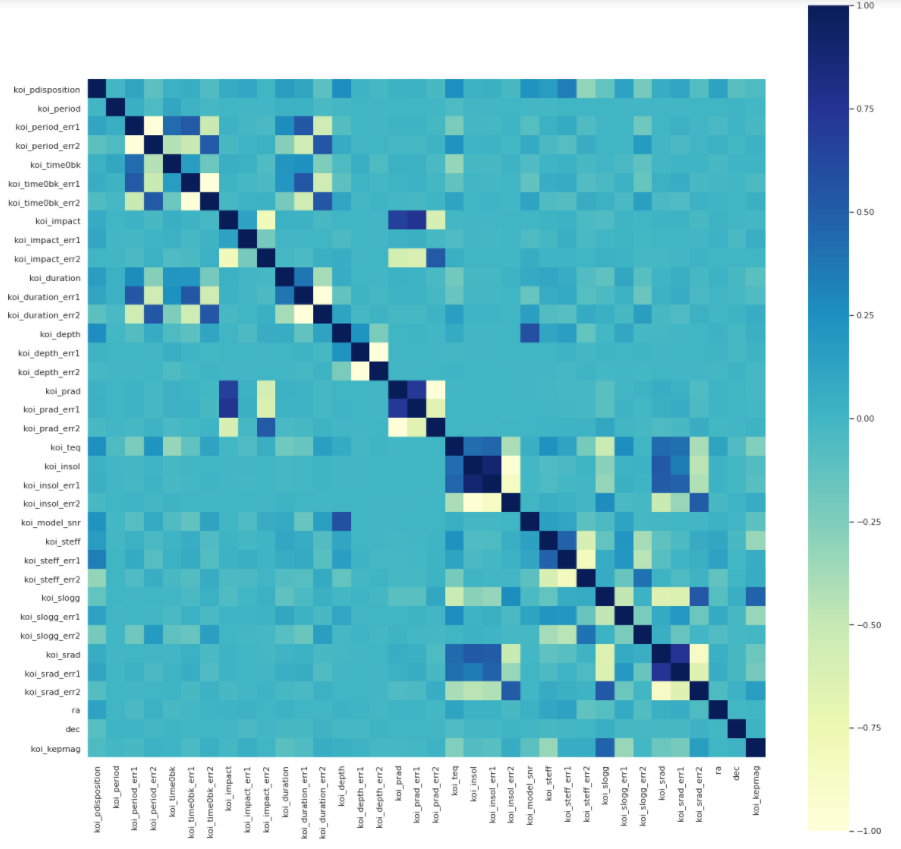
\includegraphics[scale=0.65]{pics/5.png}
\caption{Матрица корелляций}
\end{figure}

Посмотрим на распределение величин по признакам в данных:

\begin{figure}[h!]
\centering
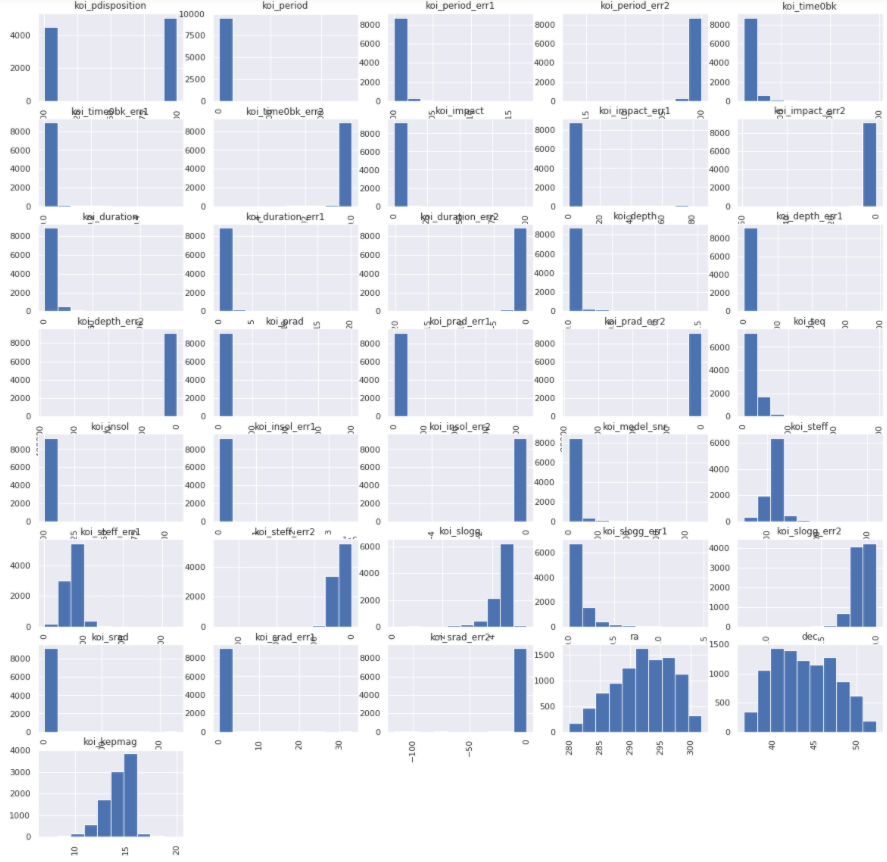
\includegraphics[scale=0.6]{pics/6.png}
\caption{Распределение величин по признакам}
\end{figure}

Для заполнения пропущенных данных используем Imputation. Imputation заполняет недостающее значение некоторым числом.

\begin{figure}[h!]
\centering
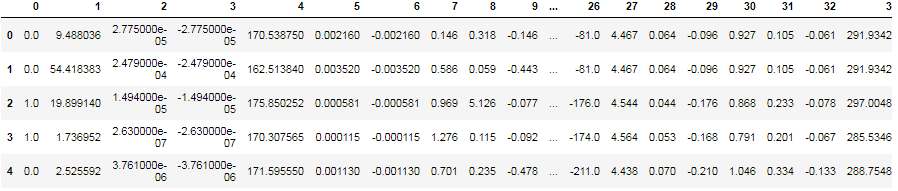
\includegraphics[scale=0.6]{pics/7.png}
\end{figure}

Создадим обучающую выборку и разделим ее на тестовую 0.15 и обучающую 0.85.

В качестве библиотеки для создания нейронных сетей  используется keras.
Задаются следующие характеристики:
\begin{enumerate}
\item на первом слое содержится 128 нейронов с relu функцией активации;
\item на втором слое содержится 64 нейронов с relu функцией активации;
\item на третьем слое содержится 64 нейрона с relu функцией активации;
\item на третьем слое содержится 64 нейрона с relu функцией активации;
\item на выходное слое содержится 1 нейрон с сигмоидной функцией;
\end{enumerate}
В качестве метода оптимизации был выбран adam. Было проведено обучение на 100 эпохах с 32 батчами

Посмотрим на графики изменения ошибки и точности по эпохе тренировочной и валидационных выборках.

\begin{figure}[h]
\begin{center}
\begin{minipage}[h]{0.45\linewidth}
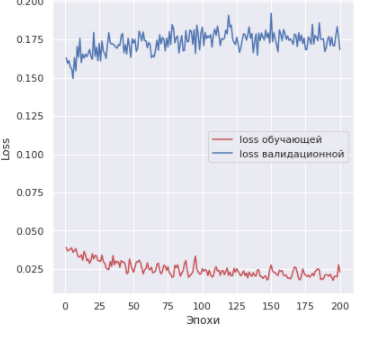
\includegraphics[width=1\linewidth]{pics/8.png}
\caption{Графики изменения ошибки}
\end{minipage}
\hfill
\begin{minipage}[h]{0.45\linewidth}
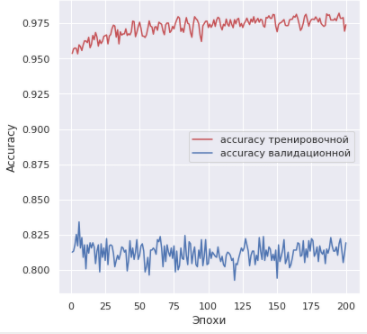
\includegraphics[width=1\linewidth]{pics/9.png}
\caption{Графики изменения точност.}
\end{minipage}
\end{center}
\end{figure}

Получим пример предсказания: 

\begin{figure}[h!]
\centering
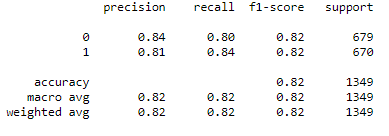
\includegraphics[scale=0.8]{pics/10.png}
\caption{Пример предсказания}
\end{figure}

\section{Вывод}
В результате данной работы была написана и обучена нейронная сеть с использованием библиотеки keras для предсказывания, а также построены графики обучения.


\end{document}